\documentclass[10pt]{article}
\usepackage[utf8]{inputenc}
\usepackage[T1]{fontenc}
\usepackage{graphicx}
\usepackage[export]{adjustbox}
\graphicspath{ {./images/} }
\usepackage{amsmath}
\usepackage{amsfonts}
\usepackage{amssymb}
\usepackage{mhchem}
\usepackage{stmaryrd}
\usepackage{bbold}
\usepackage{mathrsfs}

\title{Jinchao Xu }


\author{Deep Learning Algorithms and\\
Analysis}
\date{}


\begin{document}
\maketitle

Summer 2020


\includegraphics[max width=\textwidth]{2022_01_05_15c63bf4a948497c30d9g-02}

\section{Contents}
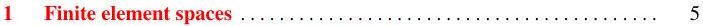
\includegraphics[max width=\textwidth]{2022_01_05_15c63bf4a948497c30d9g-03}

1.1 Conforming linear finite element spaces $\ldots \ldots \ldots \ldots \ldots \ldots \ldots$

1.1.1 Simplexes in $\mathbb{R}^{d} \ldots \ldots . . . . . . . . . . . . . . . . . . . . . . . .$

$1.1 .2$ Shape-regular and quai-uniform triangulations $\ldots \ldots \ldots . .6$

1.1.3 Finite element space .................................

$1.2$ Nodal value interpolant $\ldots \ldots \ldots \ldots \ldots \ldots \ldots \ldots, \ldots \ldots$

$1.3$ Error estimates $\ldots \ldots \ldots \ldots \ldots \ldots \ldots \ldots \ldots \ldots \ldots \ldots$


\includegraphics[max width=\textwidth]{2022_01_05_15c63bf4a948497c30d9g-04}

\section{Finite element spaces}
\subsection{Conforming linear finite element spaces}
A conforming linear finite element function in a domain $\Omega \subset \mathbb{R}^{d}$ is a continuous function that is piecewise linear function with a grid or mesh consisting of a union of simplexes.

$x_{0}$

$x_{j}$

$x_{N+1}$

Fig. 1.1. 1D uniform grid

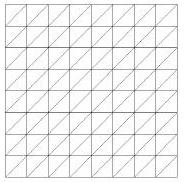
\includegraphics[max width=\textwidth]{2022_01_05_15c63bf4a948497c30d9g-05}

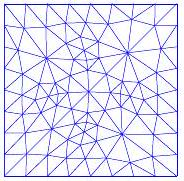
\includegraphics[max width=\textwidth]{2022_01_05_15c63bf4a948497c30d9g-05(1)}

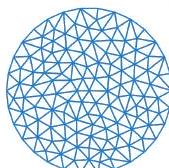
\includegraphics[max width=\textwidth]{2022_01_05_15c63bf4a948497c30d9g-05(2)}

$12 * x$

Fig. 1.2. $2 \mathrm{D}$ grids

\subsubsection{Simplexes in $\mathbb{R}^{d}$}
Let $\boldsymbol{x}_{i}=\left(x_{1, i}, \cdots, x_{d, i}\right)^{t}, i=1, \cdots, d+1$ be $d+1$ points in $\mathbb{R}^{d}$ which do not all lie in one hyper-plane. The convex hull of the $d+1$ points $\boldsymbol{x}_{1}, \cdots, \boldsymbol{x}_{d+1}$ (See Figure 1.3)
$$
\tau:=\left\{\boldsymbol{x}=\sum_{i=1}^{d+1} \lambda_{i} \boldsymbol{x}_{i} \mid 0 \leq \lambda_{i} \leq 1, i=1: d+1, \sum_{i=1}^{d+1} \lambda_{i}=1\right\}
$$
is defined as a geometric $d$-simplex generated (or spanned) by the vertices $\boldsymbol{x}_{1}, \cdots, \boldsymbol{x}_{d+1} .$ For example, a triangle is a 2-simplex and a tetrahedron is a 3-simplex. For an integer $0 \leq m \leq d-1$, an $m$-dimensional face of $\tau$ is any $m$-simplex generated by $m+1$ of the vertices of $\tau$. Zero-dimenisonal faces are vertices and one-dimensional faces are called edges of $\tau .$ The $(d-1)$-face opposite to the vertex $\boldsymbol{x}_{i}$ will be denoted by $F_{i}$.

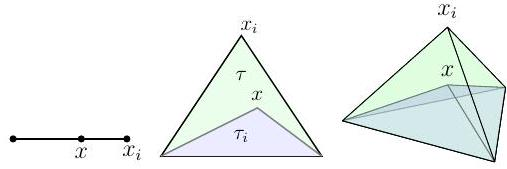
\includegraphics[max width=\textwidth]{2022_01_05_15c63bf4a948497c30d9g-06}

Fig. 1.3. Geometric explanation of barycentric coordinate

\section{Barycentric coordinates}
The numbers $\lambda_{1}(\boldsymbol{x}), \cdots, \lambda_{d+1}(\boldsymbol{x})$ are called barycentric coordinates of $\boldsymbol{x}$ with respect to the $d+1$ points $\boldsymbol{x}_{1}, \cdots, \boldsymbol{x}_{d+1}$. There is a simple geometric meaning of the barycentric coordinates. Given a $\boldsymbol{x} \in \tau$, let $\tau_{i}(\boldsymbol{x})$ be the simplex with vertices $\boldsymbol{x}_{i}$ replaced by $x$. Then it can be easily shown that
$$
\lambda_{i}(\boldsymbol{x})=\left|\tau_{i}(\boldsymbol{x})\right| /|\tau|
$$
where $|\cdot|$ is the Lebesgure measure in $\mathbb{R}^{d}$, namely area in two dimensions and volume in three dimensions. Note that $\lambda_{i}(\boldsymbol{x})$ is affine function of $\boldsymbol{x}$ and vanishes on the face $F_{i}$. We list the four basic properties of barycentric coordinate below:

    \begin{enumerate}
      \item $0 \leq \lambda_{i}(x) \leq 1$;

      \item $\sum_{i=1}^{d+1} \lambda_{i}=1$

      \item $\lambda_{i} \in P_{1}(\tau)$

      \item $\lambda_{i}\left(\boldsymbol{x}_{j}\right)=\delta_{i j} .$

    \end{enumerate}
\subsubsection{Shape-regular and quai-uniform triangulations}
Given a bounded polyhedral domain $\Omega \subset R^{d}$. A geometric triangulation (also called mesh or grid) $\mathcal{T}$ of $\Omega$ is a set of $d$-simplices such that
$$
\cup \tau=\bar{\Omega}, \quad \text { and } \quad{ }_{\tau}^{\circ} \cap{\tau}_{j}^{\circ}=\varnothing
$$
Examples of triangulations for $\Omega=(0,1)(d=1)$ are shown in Figure $1.1$ for $\Omega=$ $(0,1)(d=1)$ and Figure $1.1$ for $\Omega=(0,1)^{2}(d=2)$. Denote
$$
h_{\tau}=\operatorname{diam}(\tau), h=\max _{\tau \in \mathcal{T}_{h}} h_{\tau} ; \quad h=\min _{\tau \in \mathcal{T}_{h}} h_{\tau}
$$
The first requirement is a topological property. A triangulation $\mathcal{T}$ is called conforming or compatible if the intersection of any two simplexes $\tau$ and $\tau^{\prime}$ in $\mathcal{T}^{\prime}$ is either empty or a common lower dimensional simplex (nodes in two dimensions, nodes and edges in three dimensions).

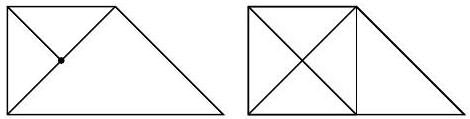
\includegraphics[max width=\textwidth]{2022_01_05_15c63bf4a948497c30d9g-07}

Fig. 1.4. Two triangulations. The left is non-conforming and the right is conforming.

The second important condition depends on the geometric structure. A set of triangulations $\mathscr{T}$ is called shape regular if there exists a constant $c_{0}$ such that
$$
\max _{\tau \in \mathcal{T}} \frac{\operatorname{diam}(\tau)^{d}}{|\tau|} \leq c_{0}, \quad \forall \mathcal{T} \in \mathscr{T}
$$
where $\operatorname{diam}(\tau)$ is the diameter of $\tau$ and $|\tau|$ is the measure of $\tau$ in $\mathbb{R}^{d}$. This assumption can also be represented as
$$
\sup _{h \in \mathbb{N}} \max _{\tau \in \mathcal{T}_{h}} \frac{h_{\tau}}{\rho_{\tau}} \leq \sigma_{1}
$$
where $\rho_{\tau}$ denotes the radius of the ball inscribed in $\tau$. In two dimensions, it is equivalent to the minimal angle of each triangulation is bounded below uniformly in the shape regular class. We shall define $h_{\tau}=|\tau|^{1 / n}$ for any $\tau \in \mathcal{T} \in \mathscr{T} .$ By (1.3), $h_{\tau} \approx \operatorname{diam}(\tau)$ represents the size of an element $\tau \in \mathcal{T}$ for a shape regular triangulation $\mathcal{T} \in \mathscr{T}$.

In addition to $(1.3)$, if
$$
\frac{\max _{\tau \in \mathcal{T}}|\tau|}{\min _{\tau \in \mathcal{T}}|\tau|} \leq \rho, \quad \forall \mathcal{T} \in \mathscr{T},
$$
$\mathscr{T}$ is called quasi-uniform. For quasi-uniform grids, $h_{\mathcal{T}}:=\max _{\tau \in \mathcal{T}} h_{\tau}$, the mesh size of $\mathcal{T}$, is used to measure the approximation rate. In the FEM literature, we often write as $\mathcal{T}_{h}$.

The assumption (1.4) is a local assumption, as is meant by above definition, for $d=2$ for example, it assures that each triangle will not degenerate into a segment in the limiting case. A triangulation satisfying this assumption is often called to be shape regular. On the other hand, the assumption (1.5) is a global assumption, which says that the smallest mesh size is not too small compared with the largest mesh size of the same triangulation. By the definition, in a quasiuniform triangulation, all the elements are about the same size asymptotically.

Remark 1 . In this course, unless otherwise noted, we restrict ourself to quasi-uniform simplicial triangulation. There are other type of meshes by partition the domain into quadrilateral (in 2-D), cubes (in 3-D), or other type of elements.

\subsubsection{Finite element space}
Given a shape regular triangulation $\mathcal{T}_{h}$ of $\Omega$, we set
$$
V_{h}:=\left\{v \mid v \in C(\bar{\Omega}), \text { and }\left.v\right|_{\tau} \in P_{1}(\tau), \forall \tau \in \mathcal{T}_{h}\right\}
$$
where $P_{1}(\tau)$ denotes the space of polynomials of degree 1 (linear) on $\tau \in \mathcal{T}_{h}$. Whenever we need to deal with boundary conditions, we further define $V_{h, 0}=V_{h} \cap H_{0}^{1}(\Omega)$.

We note here that the global continuity is also necessary in the definition of $V_{h}$ in the sense that if $u$ has a square interable gradient, that is $u \in H^{1}(\Omega)$, and $u$ is piecewise smooth, then $u$ is continuous.

We always use $n_{h}$ to denote the dimension of finite element spaces. For $V_{h}, n_{h}$ is the number of vertices of the triangulation $\mathcal{T}_{h}$ and for $V_{h, 0}, n_{h}$ is the number of interior vertices.

\section{Nodal basis functions and dual basis}
For linear finite element spaces, we have the so called a standard nodal basis functions $\left\{\varphi_{i}, i=1, \cdots n_{h}\right\}$ such that $\varphi_{i}$ is piecewise linear (with respect to the triangulation) and $\varphi_{i}\left(x_{j}\right)=\delta_{i, j} .$ Note that $\left.\varphi_{i}\right|_{\tau}$ is the corresponding barycentrical coordinates of $x_{i} .$ See Figure $1.5$ for an illustration in 2-D.

Let $\left(\psi_{i}\right)_{i=1}^{n_{h}}$ be the dual basis of $\left(\varphi_{i}\right)_{i=1}^{n_{h}} .$ Namely
$$
\left(\psi_{i}, \varphi_{j}\right)=\delta_{i, j}, \quad i, j=1, \ldots, n_{h}
$$
We notice that all the nodal basis functions $\left\{\varphi_{i}\right\}$ are locally supported, but their dual basis functions $\left\{\psi_{i}\right\}$ are in general not locally supported. The nodal basis functions $\left\{\varphi_{i}\right\}$ are easily constructed in terms of barycentric coordinate functions. The dual basis $\left\{\psi_{i}\right\}$ are only interesting for theoretical consideration and it is not necessary to know the actual constructions of these functions.

Therefore for any $v_{h} \in V_{h}$, we have the representation
$$
v_{h}(x)=\sum_{i=1}^{n_{h}} v_{h}\left(x_{i}\right) \varphi_{i}(x)
$$
Let us see how our construction looks like in one spatial dimension. Associated with the partition $\mathcal{T}_{h}=\left\{0=x_{0}<x_{1}<\ldots<x_{n_{h}}<x_{n_{h}+1}=1\right\}$, we define a linear finite element space\\

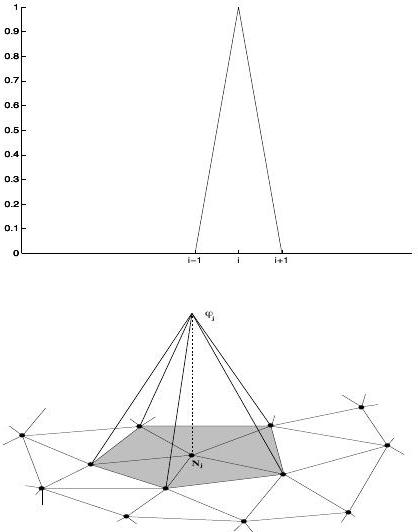
\includegraphics[max width=\textwidth]{2022_01_05_15c63bf4a948497c30d9g-09}

Fig. 1.5. Nodal basis functions in $1 \mathrm{~d}$ and $2 \mathrm{~d}$

$V_{h, 0}=\left\{v: v\right.$ is continuous and piecewise linear w. r. t. $\left.\mathcal{T}_{h}, v(0)=v(1)=0\right\} .$

A plot of a typical element of $V_{h, 0}$ is shown in Fig. 1.6.

It is easily calculated (as we already mentioned), that the dimension of $V_{h}$ is equal to the number of internal vertices, and the nodal basis functions spanning $V_{h, 0}$ (for $\left.i=1,2, \cdots, n_{h}\right)$ are (see also Fig. 1.5):
$$
\varphi_{i}(x)=\left\{\begin{array}{cl}
\frac{x-x_{i-1}}{h}, & x \in\left[x_{i-1}, x_{i}\right] \\
\frac{x_{i+1}-x}{h}, & x \in\left[x_{i}, x_{i+1}\right] \\
0 & \text { elsewhere }
\end{array}\right.
$$

\subsection{Nodal value interpolant}
Lemma 1. For any $v \in V_{h}$,
$$
v(x)=\sum_{j=1}^{N_{h}} v\left(x_{j}\right) \phi_{j}(x)
$$
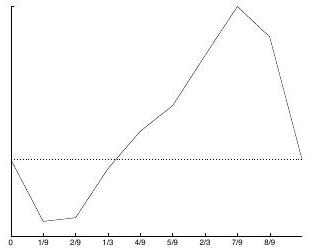
\includegraphics[max width=\textwidth]{2022_01_05_15c63bf4a948497c30d9g-10}

Fig. 1.6. Plot of a typical element from $V_{h}$.

Proof. Let $v_{h}(x)=\sum_{j=1}^{N_{h}} v\left(x_{j}\right) \phi_{j}(x) .$ For an arbitrary $\operatorname{simplex}$ with $d+1\left(\Omega \subseteq \mathbb{R}^{d}\right)$ vertices $a_{1}, \cdots, a_{d+1}$ :
$$
v_{h}(x)=\sum_{j=1}^{d+1} v\left(a_{j}\right) \lambda_{j}(x)
$$
Notice that
$$
v_{h}\left(a_{i}\right)=\sum_{j=1}^{d+1} v\left(a_{j}\right) \lambda_{j}\left(a_{i}\right)=v\left(a_{j}\right), i=1, \cdots, d+1
$$
So the values of $v_{h}$ and $v$ are equal at $d+1$ points. Notice that both $v_{h}$ and $v$ are linear functions, so $v=v_{h} . \square$

For any continuous function $u$, we define its finite element interpolation, $u_{I} \in$ $V_{h, 0}$, as follows:
$$
u_{I}(x)=\sum_{i=1}^{N} u\left(x_{i}\right) \phi_{i}(x)
$$
For any $v \in \mathcal{S}_{0}^{h}$, we can obviously write
$$
v(x)=\sum_{i=1}^{N} v\left(x_{i}\right) \phi_{i}(x)
$$
The nodal value interpolation operator $I_{h}: C(\bar{\Omega}) \mapsto V_{h}$ is defined as follows
$$
\left(I_{h} u\right)\left(x_{i}\right)=u\left(x_{i}\right), \quad \forall x_{i} \in \mathcal{N}_{h} .
$$

\subsection{Error estimates}
Theorem 1. Assume that $\left\{\mathcal{T}_{h}: h \in \aleph\right\}$ is quasiuniform, then
$$
\inf _{v_{h} \in V_{h}}\left\|v-v_{h}\right\|+h\left|v-v_{h}\right|_{1} \lesssim h^{2}|v|_{2} \quad \forall v \in H^{2}(\Omega)
$$
Next we provide proofs of the above theorem for some special cases.

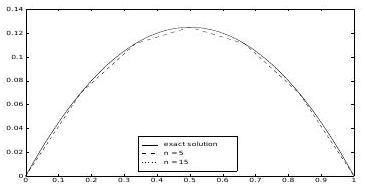
\includegraphics[max width=\textwidth]{2022_01_05_15c63bf4a948497c30d9g-11}

Fig. 1.7. Approximation of finite element space.

\section{A proof of Theorem 1 for $d=1$}
Observe first that $e=\left(u-u_{I}\right)$ vanishes at the end points of each interval and $e^{\prime}$ is continuous, because $e^{\prime \prime}$ is square integrable. By the Rolle's theorem there exists $\xi_{i} \in\left(x_{i}, x_{i+1}\right)$ such that $e^{\prime}\left(\xi_{i}\right)=0 .$ By the Fundamental Theorem of Calculus for $x \in\left(x_{i}, x_{i+1}\right)$, we have that
$$
e^{\prime}(x)=\int_{\xi_{i}}^{x} e^{\prime \prime}(t) d t
$$
Since $u_{I}$ is linear on $\left[x_{i}, x_{i+1}\right]$ we have that $e^{\prime \prime}(t)=u^{\prime \prime}(t)$, and hence
$$
\left[e^{\prime}(x)\right]^{2}=\left[\int_{\xi_{i}}^{x} u^{\prime \prime}(t) d t\right]^{2}
$$
Applying the Schwarz inequality to the right side then gives,
$$
\begin{aligned}
\left[e^{\prime}(x)\right]^{2} & \leq\left|\int_{\xi_{i}}^{x} 1^{2} d t\right|\left|\int_{\xi_{i}}^{x}\left[u^{\prime \prime}(t)\right]^{2} d t\right| \\
& \leq\left|\xi_{i}-x\right| \int_{x_{i}}^{x_{i+1}}\left[u^{\prime \prime}(t)\right]^{2} d t .
\end{aligned}
$$
Integrating from $x_{i}$ to $x_{i+1}$, and observing that
$$
\int_{x_{i}}^{x_{i+1}}\left|\xi_{i}-x\right| d x=\frac{1}{2}\left[\left(\xi_{i}-x_{i}\right)^{2}+\left(x_{i+1}-\xi_{i}\right)^{2}\right] \leq\left(x_{i}-x_{i+1}\right)^{2},
$$
then gives
$$
\int_{x_{i}}^{x_{i+1}}\left[e^{\prime}(x)\right]^{2} d x \leq\left(x_{i+1}-x_{i}\right)^{2} \int_{x_{i}}^{x_{i+1}}\left[u^{\prime \prime}(t)\right]^{2} d t .
$$
Finally, summing up on $(0,1)$ then leads to:
$$
\begin{aligned}
\left\|e^{\prime}\right\|_{0, \Omega}=\int_{0}^{1}\left[e^{\prime}(x)\right]^{2} d x &=\sum_{i=1}^{n_{h}-1} \int_{x_{i}}^{x_{i+1}}\left[e^{\prime}(x)\right]^{2} d x \\
& \leq \sum_{i=1}^{n_{h}-1}\left(x_{i+1}-x_{i}\right)^{2} \int_{x_{i}}^{x_{i+1}}\left[u^{\prime \prime}(t)\right]^{2} d t \\
& \leq \max _{i}\left(x_{i+1}-x_{i}\right)^{2} \int_{0}^{1}\left[u^{\prime \prime}(t)\right]^{2} d t
\end{aligned}
$$
Since $e\left(x_{i}\right)=0$, for any $x \in\left(x_{i}, x_{i+1}\right)$,
$$
|e(x)|=\left|\int_{x_{i}}^{x} e^{\prime}(t) d t\right| \lesssim h|e|_{1, \tau} \lesssim h^{2}|u|_{2, \tau} .
$$
Summing up on $(0,1)$ then leads to:
$$
\|e\|_{0, \Omega} \lesssim h^{2}|u|_{2, Q} .
$$
This completes the proof of the estimate in one dimension.

A proof of Theorem 1 for $d=1,2,3$

Let $x=\left(x^{1}, \ldots, x^{d}\right)$ and $a_{i}=\left(a_{i}^{1}, \ldots, a_{i}^{d}\right) .$ Introducing the auxiliary functions
$$
g_{i}(t)=v\left(a_{i}(t)\right), \text { with } a_{i}(t)=a_{i}+t\left(x-a_{i}\right),
$$
we have
$$
g_{i}^{\prime}(t)=(\nabla v)\left(a_{i}(t)\right) \cdot\left(x-a_{i}\right)=\sum_{l=1}^{d}\left(\partial_{l} v\right)\left(a_{i}(t)\right)\left(x^{l}-a_{i}^{l}\right)
$$
and
$$
\left.g_{i}^{\prime \prime}(t)=\sum_{k, l=1}^{d} \partial_{k l}^{2} v\right)\left(a_{i}(t)\right)\left(x^{k}-a_{i}^{k}\right)\left(x^{l}-a_{i}^{l}\right)
$$
By Taylor expansion
$$
g_{i}(0)=g_{i}(1)-g_{i}^{\prime}(1)+\int_{0}^{1} t g_{i}^{\prime \prime}(t) d t
$$
Namely
$$
v\left(a_{i}\right)=v(x)-(\nabla v)(x) \cdot\left(x-a_{i}\right)+\int_{0}^{1} t g_{i}^{\prime \prime}(t) d t
$$
Note that
$$
\left(I_{h} v\right)(x)=\sum_{i=1}^{n+1} v\left(a_{i}\right) \lambda_{i}(x), \sum_{i=1}^{n+1} \lambda_{i}(x)=1
$$
and
$$
\sum_{i=1}^{n+1}\left(x-a_{i}\right) \lambda_{i}(x)=0
$$
It follows that
$$
\left(I_{h} v-v\right)(x)=\sum_{i=1}^{n+1} \lambda_{i}(x) \int_{0}^{1} t g_{i}^{\prime \prime}(t) d t
$$
Using (1.9) and the trivial fact that $\left|x^{l}-a_{i}^{l}\right| \leq h$, we obtain
$$
\left\|g_{i}^{\prime \prime}(t)\right\|_{L^{2}(\tau)} \leq h^{2} \sum_{k, l=1}^{d}\left\|\left(\partial_{k l}^{2} v\right)\left(a_{i}(t)\right)\right\|_{L^{2}\left(\tau_{i}^{\prime}\right)} \leq h^{2} t^{-n / 2} \sum_{k, l=1}^{d}\left\|\partial_{k l}^{2} v\right\|_{L^{2}(\tau)}
$$
where we have used the following change of variable
$$
y=a_{i}+t\left(x-a_{i}\right): \tau \mapsto \tau_{i}^{t} \subset \tau \text { with } d y=t^{d} d x
$$
Now taking the $L^{2}(\tau)$ norm on both hand of sides of $(1.11)$, we get
$$
\begin{aligned}
\left\|I_{h} v-v\right\|_{L^{2}(\tau)} & \leq h^{2} \sum_{i=1}^{n+1} \max _{x \in \tau}\left|\lambda_{i}(x)\right| \int_{0}^{1} t\left\|g_{i}^{\prime \prime}(t)\right\|_{L^{2}(\tau)} d t \\
& \leq(n+1) \int_{0}^{1} t^{1 / n / 2} d t h^{2} \sum_{k, l=1}^{d}\left\|\partial_{k l}^{2} v\right\|_{L^{2}(\tau)} \\
& \leq \frac{2(n+1)}{4-n} h^{2} \sum_{k, l=1}^{d}\left\|\partial_{k l}^{2} v\right\|_{L^{2}(\tau)} \\
& \leq \frac{4 n(n+1)}{4-n} h^{2}|v|_{H^{2}(\tau)}
\end{aligned}
$$
Now we prove the $H^{1}$ error estimate. Notice that
$$
\left[\partial_{j}\left(I_{h} v-v\right)\right](x)=\sum_{i}\left(\partial_{j} \lambda_{i}\right)(x) \int_{0}^{1} t g_{i}^{\prime \prime}(t) d t+\sum_{i} \lambda_{i}(x) \partial_{j} \int_{0}^{1} t g_{i}^{\prime \prime}(t) d t
$$
By $(1.10)$,
$$
\int_{0}^{1} \operatorname{tg}_{i}^{\prime \prime}(t) d t=v\left(a_{i}\right)-v(x)+(\nabla v)(x) \cdot\left(x-a_{i}\right)
$$
therefore,
$$
\begin{aligned}
& \partial_{j} \int_{0}^{1} \operatorname{tg}_{i}^{\prime \prime}(t) d t \\
&=-\partial_{j} v+\left(\nabla \partial_{j} v\right)(x)\left(x-a_{i}\right)+\nabla v \cdot e_{j} \quad\left(e_{j} \text { is the } j \text {-th standard basis }\right) \\
&=\left(\nabla \partial_{j} v\right)(x)\left(x-a_{i}\right)
\end{aligned}
$$
Notice that $\sum_{i} \lambda_{i}\left(\nabla \partial_{j} v\right)(x)\left(x-a_{i}\right)=0$ :
$$
\left[\partial_{j}\left(I_{h} v-v\right)\right](x)=\sum_{i}\left(\partial_{j} \lambda_{i}\right)(x) \int_{0}^{1} t g_{i}^{\prime \prime}(t) d t
$$
Then the estimate for $\left|\nabla\left(I_{h} v-v\right)\right|_{L^{2}(\tau)}$ follows by a similar argument and the following obvious estimate
$$
\left|\left(\nabla \lambda_{i}\right)(x)\right| \lesssim \frac{1}{h}
$$
On the proof of Theorem 3 for $d \geq 4$

The above proof using interpolation for Theorem 3 does not apply for $d \geq 4 .$ This is because when $d \geq 4$, the embedding relation between $H^{2}(\Omega)$ and $C(\bar{\Omega})$ is not true. Only continuous functions can have interpolations. In this case, one approach is to use the so-called Scott-Zhang interpolation ?, the details can be found in ?.

Theorem 2. Let $V_{N}$ be linear finite element space on a quasi-uniform simplicial triangulation consisting of $N$ element. Then
$$
\inf _{v_{h} \in V_{N}}\left\|v-v_{N}\right\|+h\left|v-v_{N}\right|_{1} \lesssim N^{-\frac{2}{d}}|v|_{2} \quad \forall v \in H^{2}(\Omega)
$$
We can refine and extend the above error estimate in many different ways.

Theorem 3. Given any function $v$ with certain regularity assumption (say $v \in$ $H^{2}(\Omega)$ ), then there is a shape regular grid $\mathcal{T}_{N}$ consisting of $N$ simplicial elements
$$
\inf _{v_{h} \in V_{N}}\left\|v-v_{N}\right\|+h\left|v-v_{N}\right|_{1} \leq C(v) N^{-\frac{2}{d}} .
$$
where $V_{N}$ is linear finite element space on associated with $\mathcal{T}_{N} .$

Theorem 4. ?or any function $v$ that is not locally linear, we have
$$
\inf _{\operatorname{dim} V_{N}=N} \inf _{v_{h} \in V_{N}}\left\|v-v_{N}\right\|+h\left|v-v_{N}\right|_{1} \geq c(v) N^{-\frac{2}{a}}
$$
where $V_{N}$ be linear finite element space on associated with a shape regular mesh $\mathcal{T}_{N} .$


\end{document}